\documentclass[20pt]{article}
\usepackage[paperheight=16in,paperwidth=24in,top=1in,bottom=1in,right=1in,left=1in,heightrounded]{geometry}
\usepackage[latin1]{inputenc}
\usepackage{amsmath}
\usepackage{amsfonts}
\usepackage{amssymb}
\usepackage{graphicx}
\usepackage{multicol}
\usepackage{tikz}
\usetikzlibrary{shapes.geometric, arrows}
\usepackage{framed}	

\tikzstyle{startstop} = [rectangle, rounded corners, minimum width=3cm, minimum height=1cm,text centered,text width=15cm, draw=black, fill=red!30]
\tikzstyle{io} = [trapezium, trapezium left angle=70, trapezium right angle=110, minimum width=3cm, minimum height=1cm, text centered, draw=black, fill=blue!30]
\tikzstyle{process} = [rectangle, minimum width=3cm, minimum height=1cm, text centered, draw=black, fill=orange!30]
\tikzstyle{decision} = [diamond, minimum width=3cm, minimum height=1cm, text centered, draw=black, fill=green!30]
\tikzstyle{arrow} = [thick,->,>=stealth] %TODO make thicker 


\definecolor{CMUred}{rgb}{153.0,0.0,0.0}


\usetikzlibrary{calc}

\begin{document}
% % TITLE 
\centering
 \begin{tikzpicture}[overlay, remember picture]
    \draw let \p1 = (current page.west), \p2 = (current page.east) in
      node[minimum width=\x2-\x1, minimum height=2cm, draw, rectangle, fill=CMUred, anchor=north west, align=left, text width=\x2-\x1] at ($(current page.north west)$) {\Large\bfseries \quad
      \begin{multicols}{3}
      \begin{center}

\includegraphics[width=2cm]{./ri_logo}
      \end{center}
      \begin{center}
      \textcolor{white}{
	  \Huge
      	SKEW WORDS\\
      	\normalsize
      	 by Sarah Tan, Phil Bailey, and Trevor Decker}
      	 \end{center}
      	 \columnbreak
%s
      	       \begin{center}
      	 
\includegraphics[height=2cm]{ecelogo.png}
      	       \end{center}
      \end{multicols}
      	};
  \end{tikzpicture}
.\\
.\\
.\\
\begin{tikzpicture}*[node distance=2cm]
\node (intro) [startstop,yshift=0.0cm] {Skew Words goal is to detect and read text from an image\\ From reading text on integrated circuits to be constructed to driving around on the street, robots need the ability to identify text from images. The goal of this paper is to create a robust approach to text detection in inconsistent environments. We intend to be able to read text oriented randomly whether it is on a STOP sign, on a CPU, or just written on a piece of paper. };

\node (start) [startstop,yshift=-4.5cm] {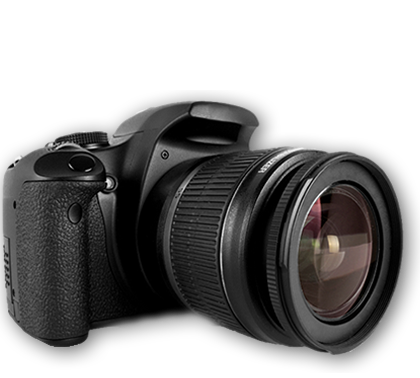
\includegraphics{camera.png}\\Take A picture with Camera, saving it as a .jpg on computer };
\node (step1) [startstop, below of=start,yshift=-3cm] {Read file into MATLAB};
% % THREASHOLD IMAGE

\node (step2) [startstop, below of=step1,yshift=-4.0cm] {{\huge Threashold the image}\\ 
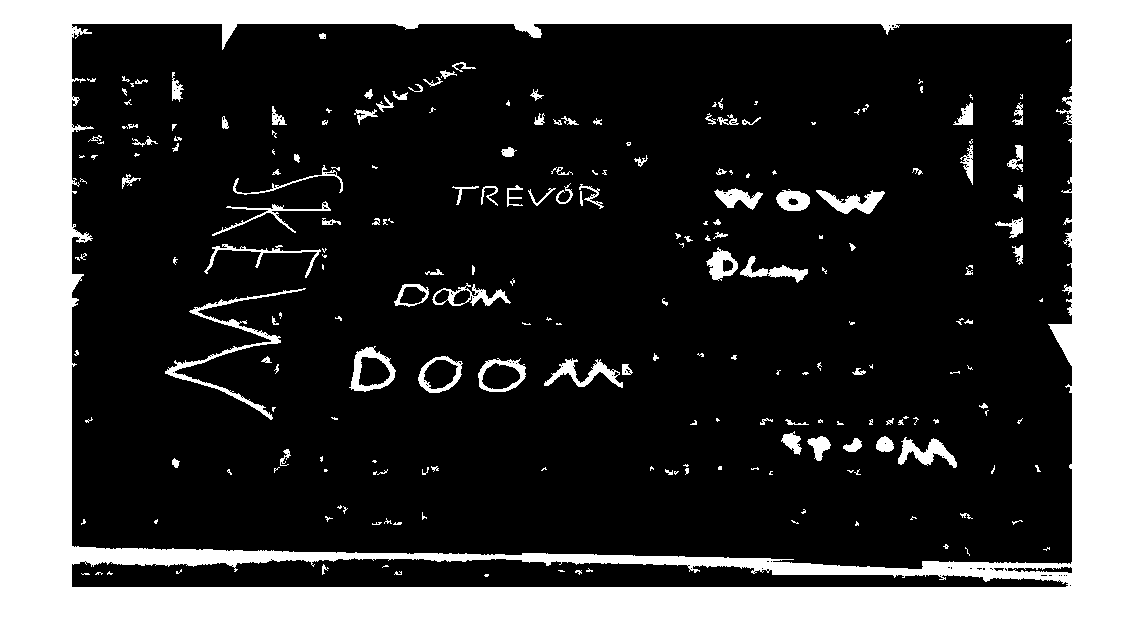
\includegraphics[width=6cm]{../thresh}
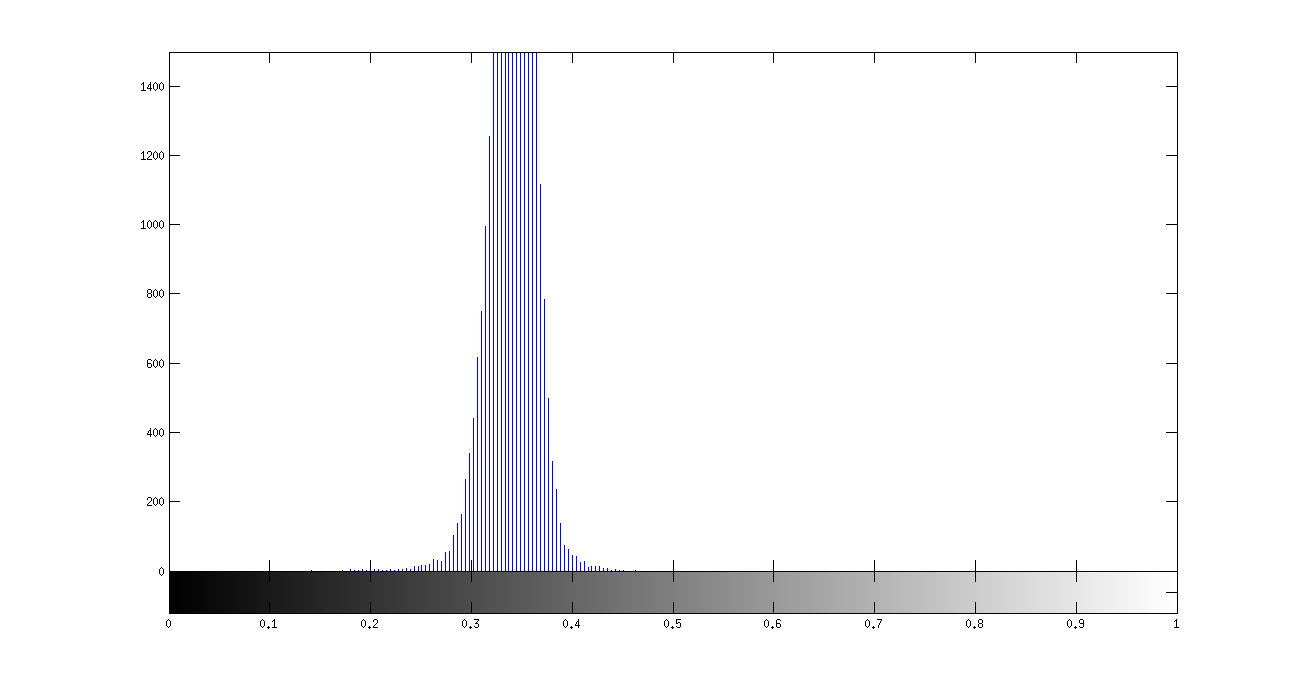
\includegraphics[width=6cm]{../th_hist}

	First we transform the image from rgb color space to its hue, saturation, value repersentation, Then We extend the border of the image to make sure that the image has a larger background region then forground region.  Next we seperate the image into ovrlapping subboxs, for each sub box we dynamicly find a threashold for the grayscale,saturation and value terms of that box.  To find the threashold we use the images color chanel histogram to find a intrest point.  
};

%Get image from camera
\node (step3) [startstop, below of=step2,yshift=-7.0cm] { {\huge Group potential letter segments}\\
\includegraphics[width=6cm]{group.png}\\
%TODO
Once we have a boolean map of pixels, as potentialy being a part of a letter or not being a part of a letter.  Pixels which could be a part of a letter and that are close to each other are combined into groups.  This is equivlent to the segmentation problem of the boolean threashold image.
};
\node (step4) [startstop, below of=step3,yshift=-6.5cm] {Rectify potential letter segments\\
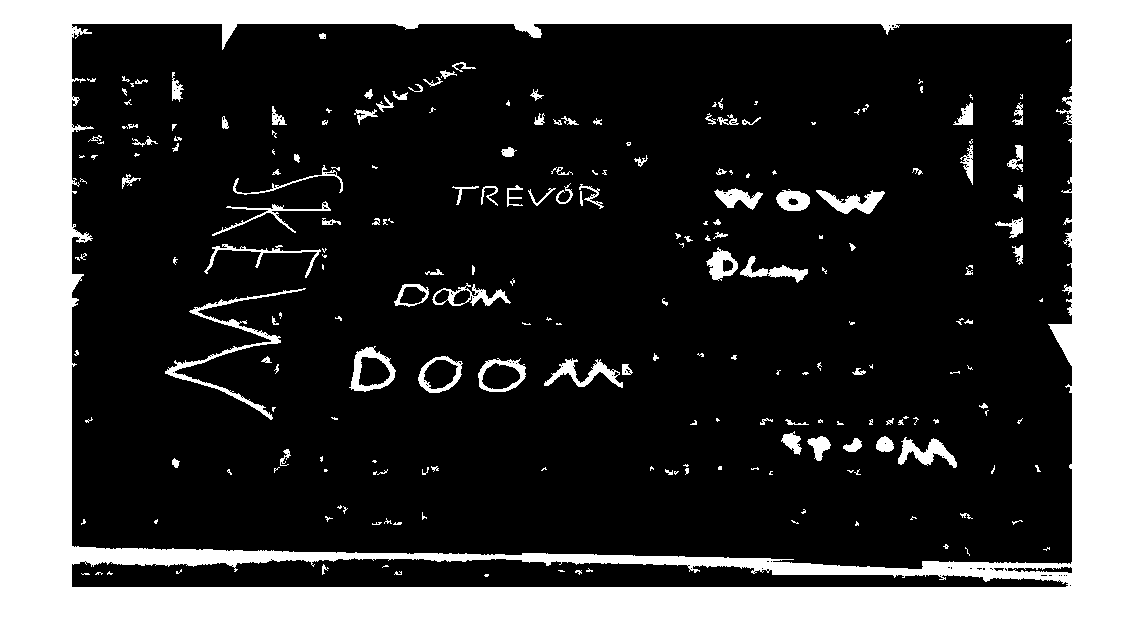
\includegraphics[width=6cm]{../thresh}
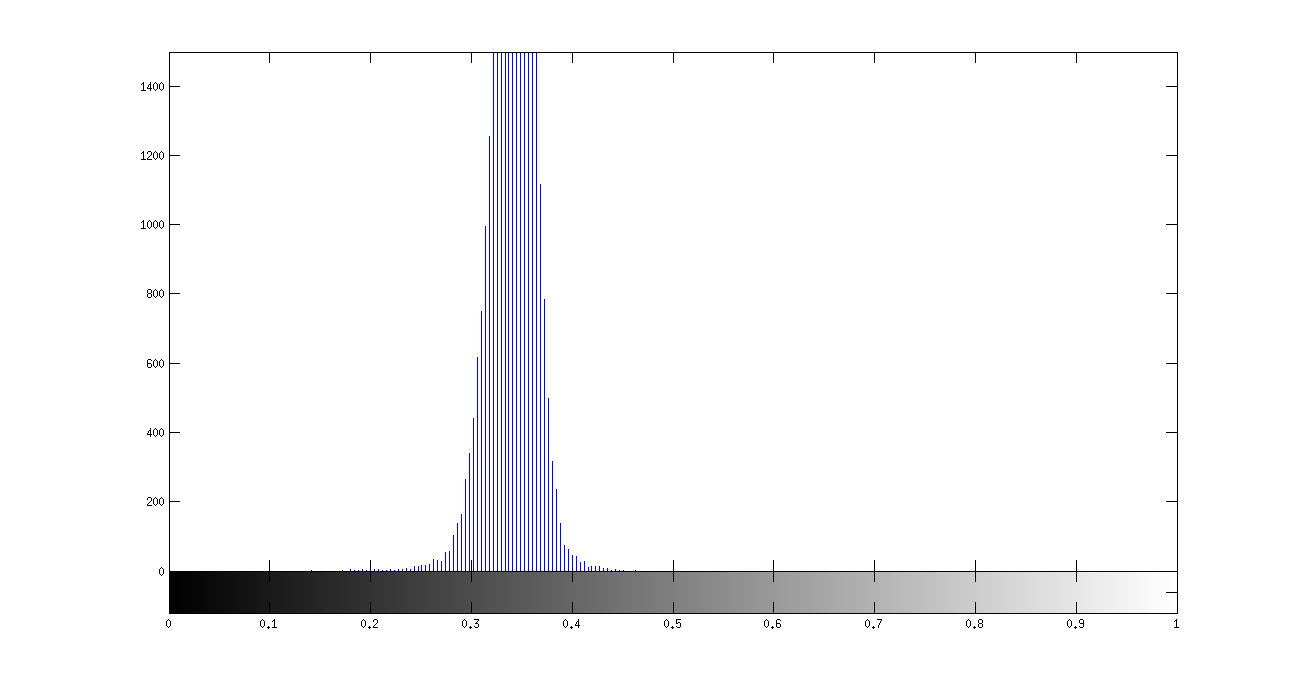
\includegraphics[width=6cm]{../th_hist}
%TODO
};
\node (step5) [startstop, below of=intro,yshift=-1cm, xshift=17cm] {test potential letter segments\\
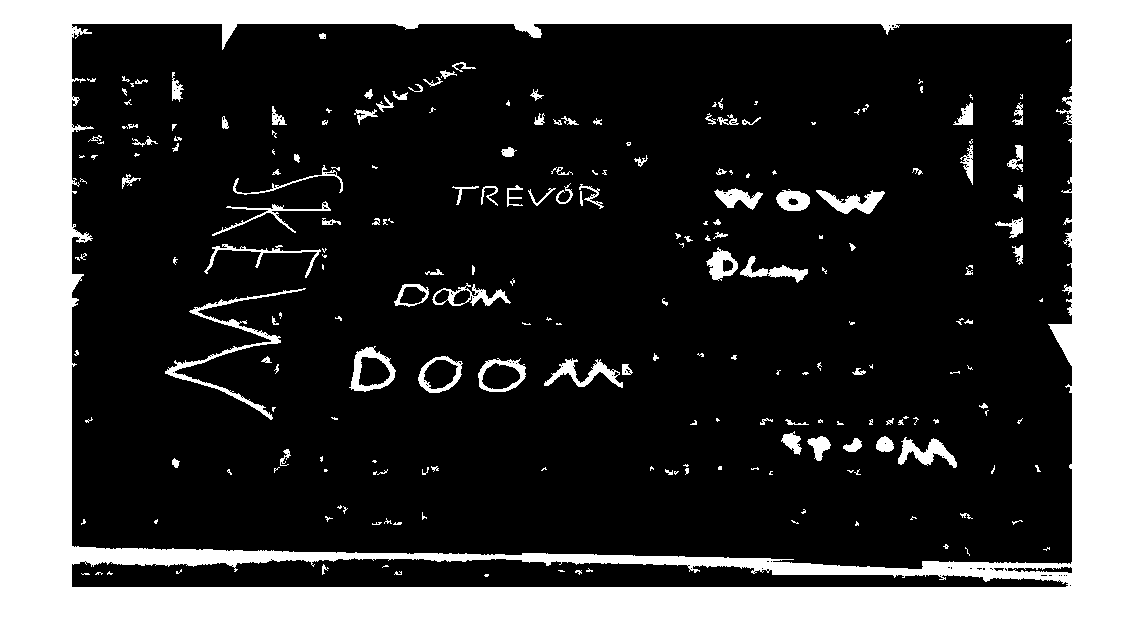
\includegraphics[width=6cm]{../thresh}
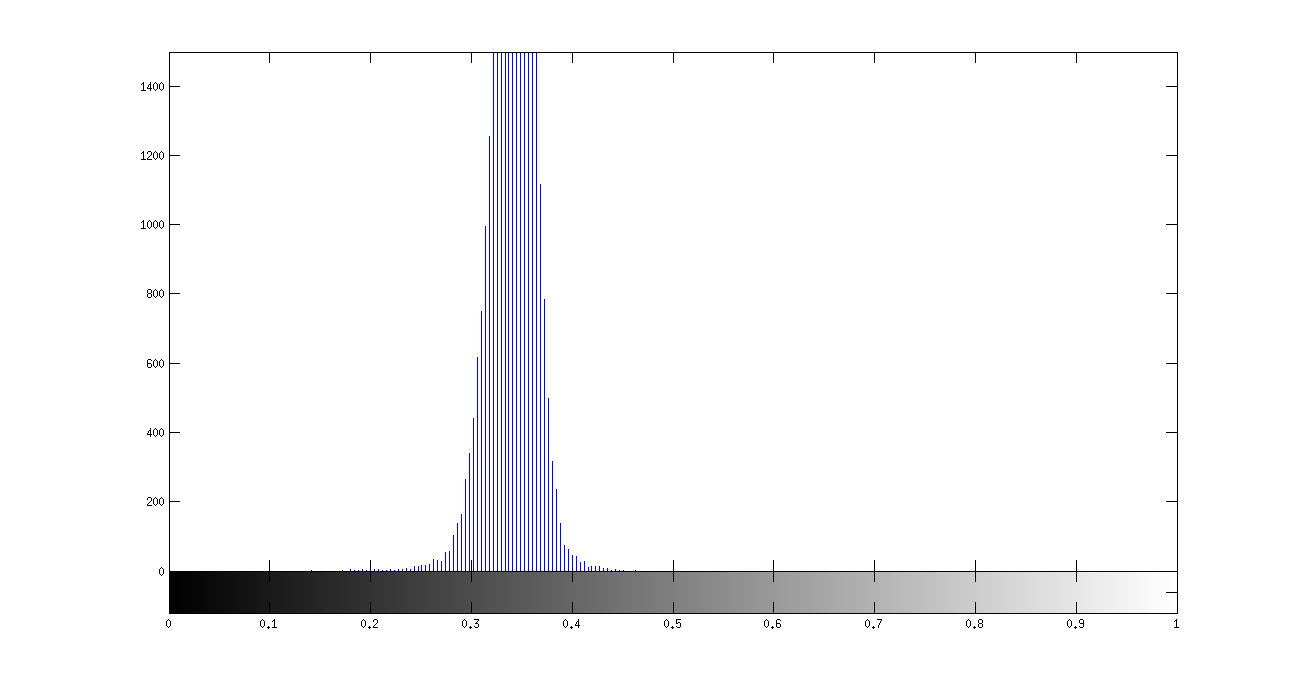
\includegraphics[width=6cm]{../th_hist}
%TODO
};
\node (step6) [startstop, below of=step5,yshift=-4.0cm] {ML stuff segments\\
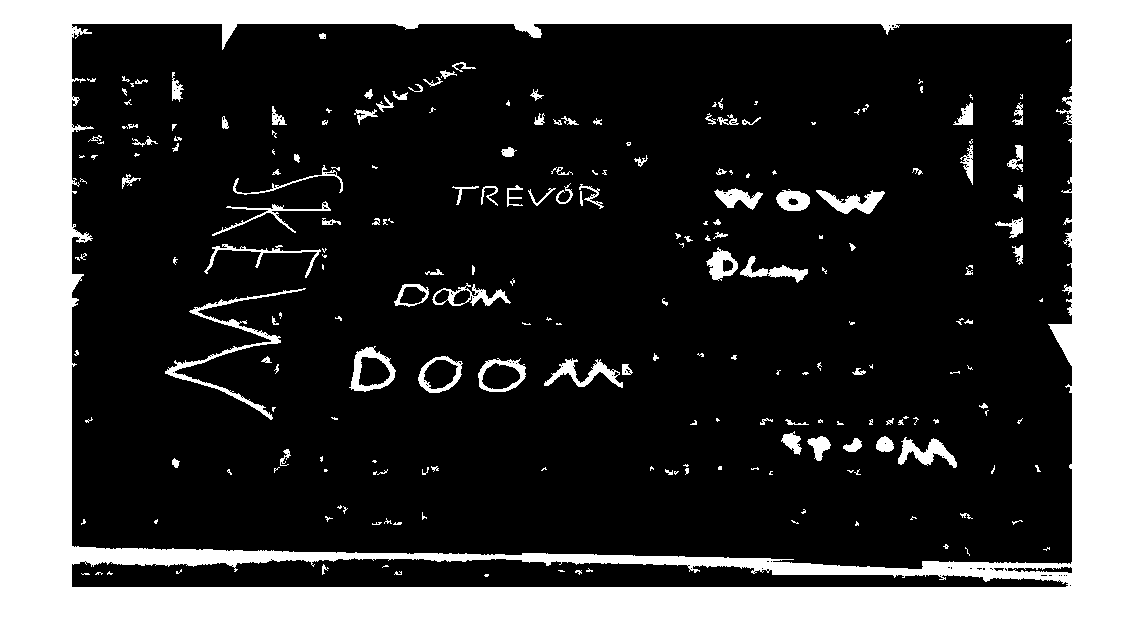
\includegraphics[width=6cm]{../thresh}
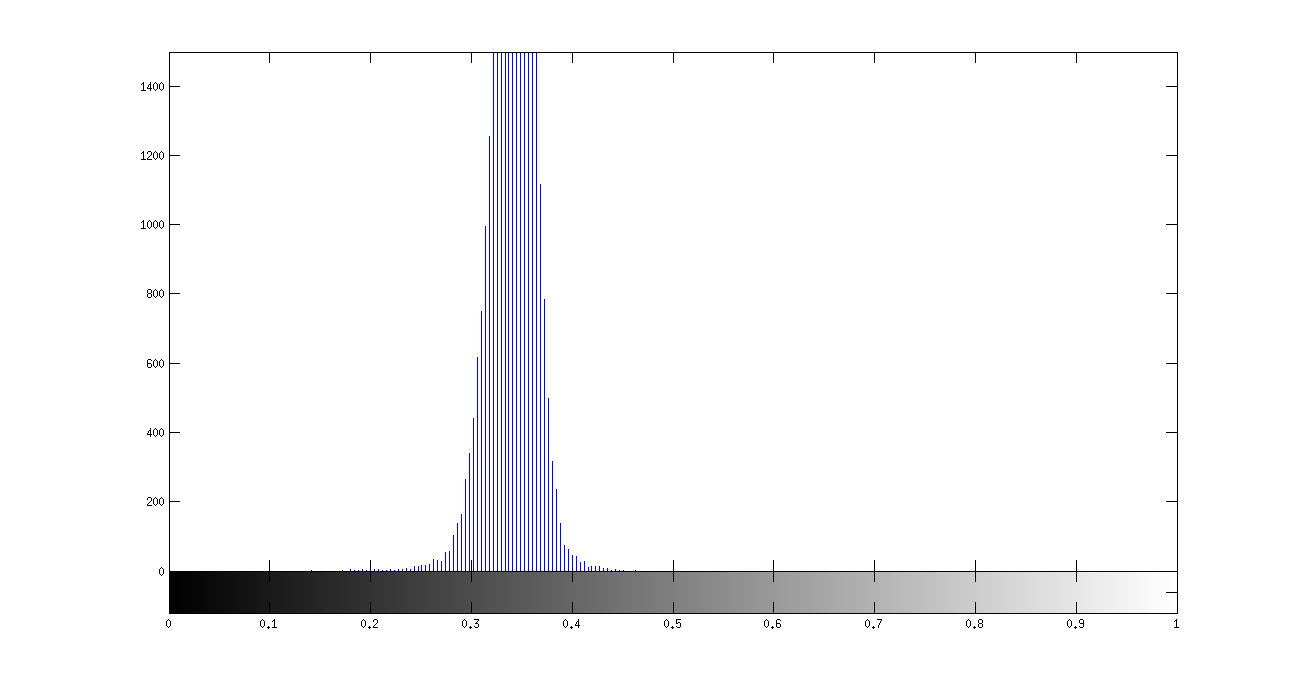
\includegraphics[width=6cm]{../th_hist}
%TODO
};
\node (step7) [startstop, below of=step6,yshift=-4.0cm] {{\huge Letter Grouping}\\ %TODO
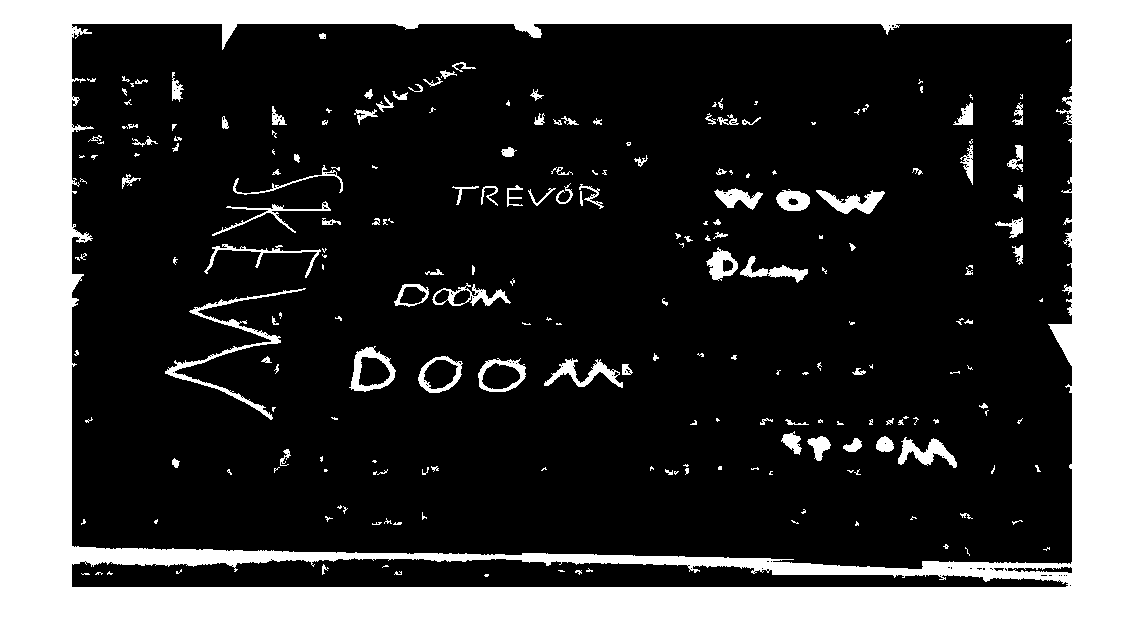
\includegraphics[width=6cm]{../thresh}
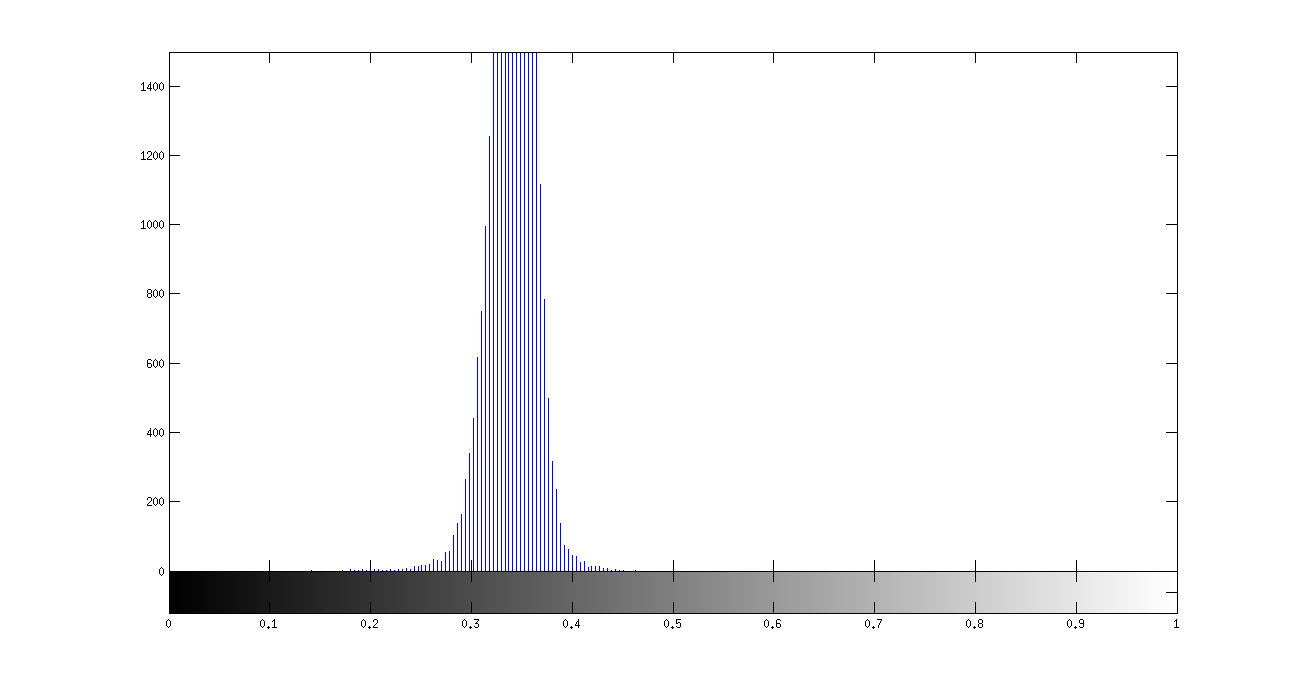
\includegraphics[width=6cm]{../th_hist}
%TODO
};
\node (step8) [startstop, below of=step7,yshift=-4.0cm] {{\huge Dictionary Data validation}\\ 

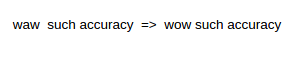
\includegraphics{dict.png}

To produce words from our estimated letters we pick the most likely combination of letters by seeing the how close each possible word combination is to a word in the dictionary, taking in to account the probability with which we detected each letter.  We also run the letters backwards in case the word is flipped.\\

  };
\node (step9) [startstop, below of=step8,yshift=-2cm] {{\huge output}\\,We then select the most likely choice for each word and return it as text to the user};

\node(result) [startstop,below of=step5,yshift = -4.5cm,xshift=17cm]{ {\huge Results} \\
explation 1 \\%TODO 
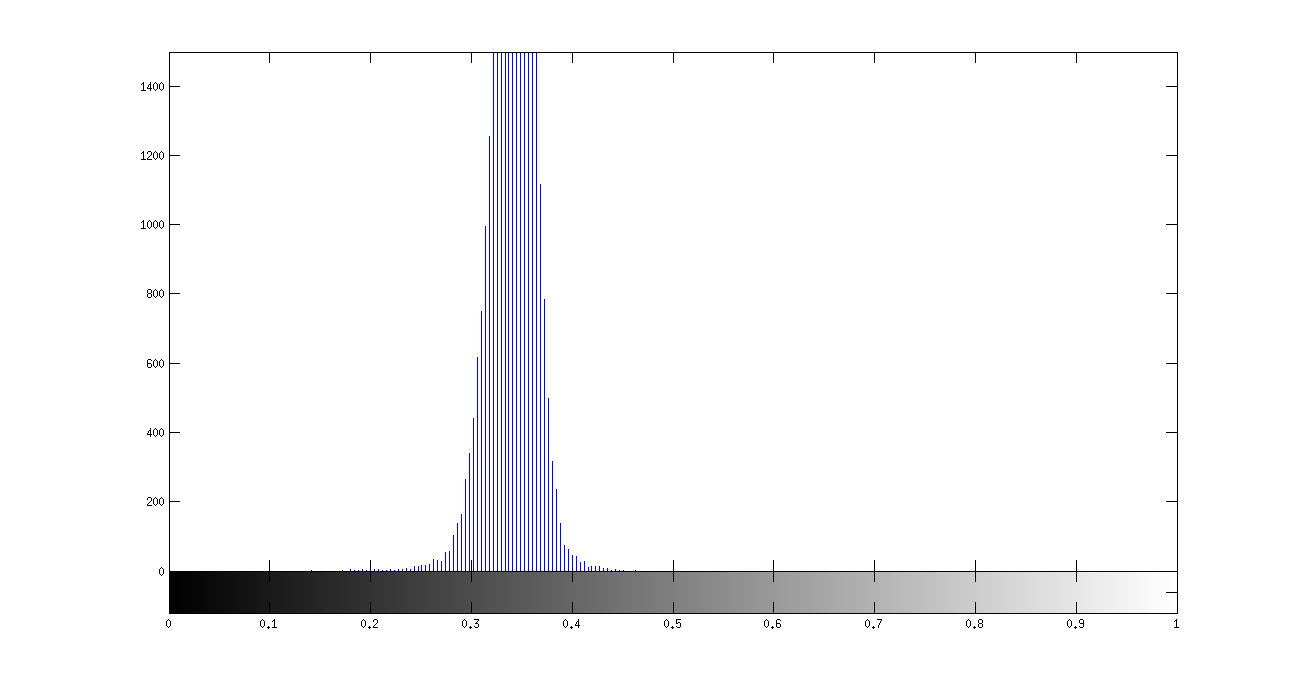
\includegraphics[width=6cm]{../th_hist}\\
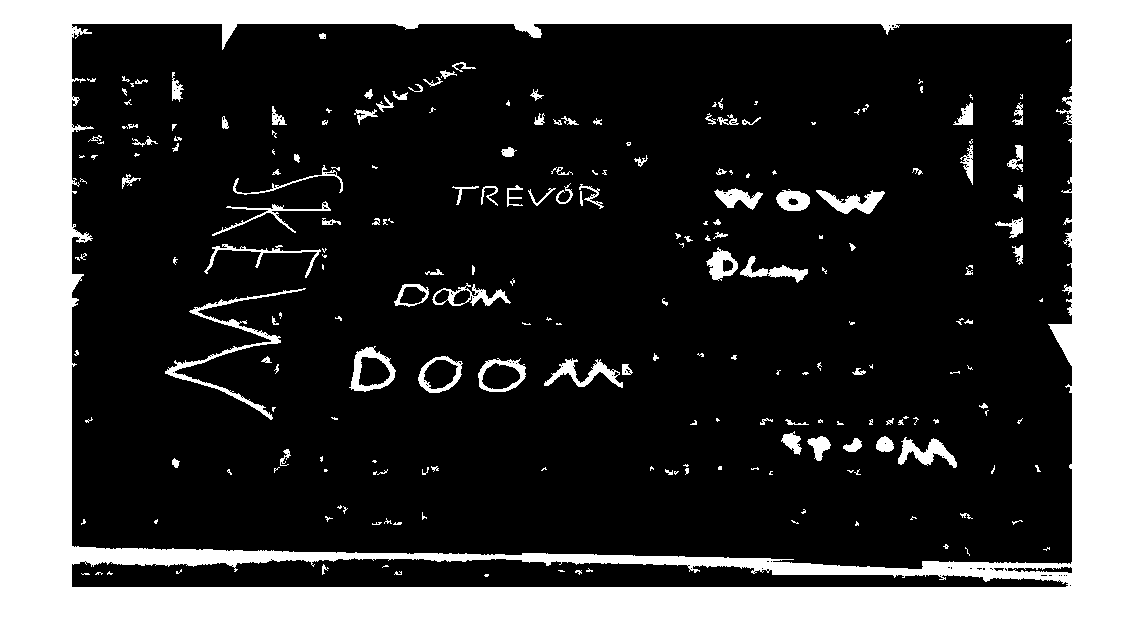
\includegraphics[width=6cm]{../thresh}\\
We compared our method of text detection to MATLABS built in optical Character recognition\\
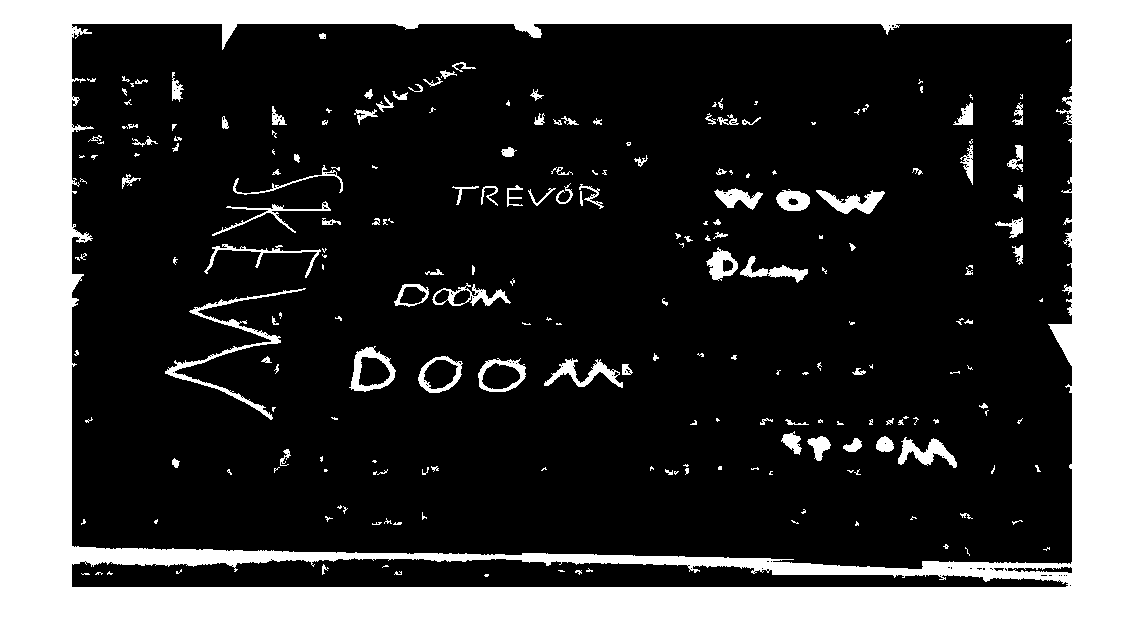
\includegraphics[width=6cm]{../thresh}
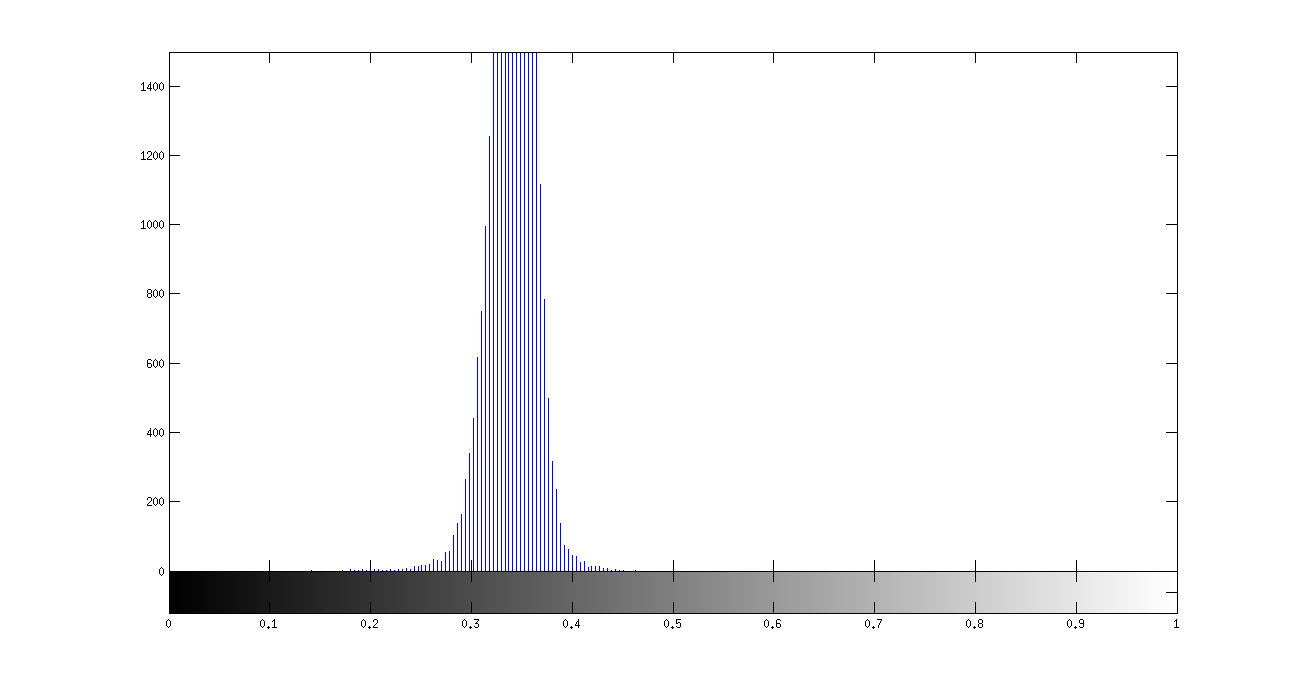
\includegraphics[width=6cm]{../th_hist}\\
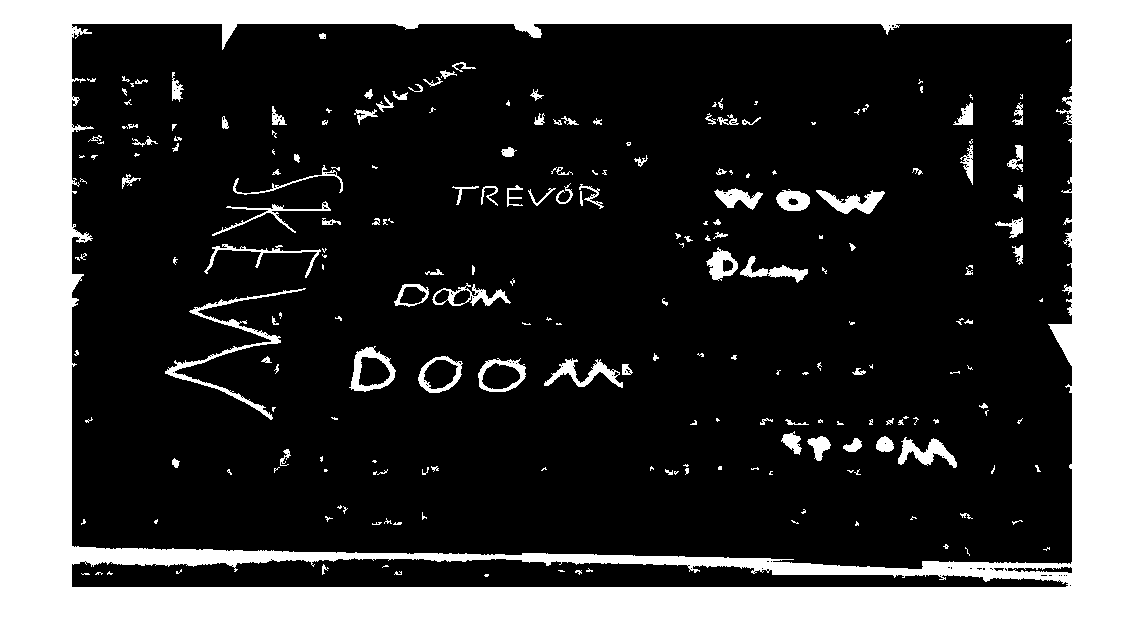
\includegraphics[width=6cm]{../thresh}
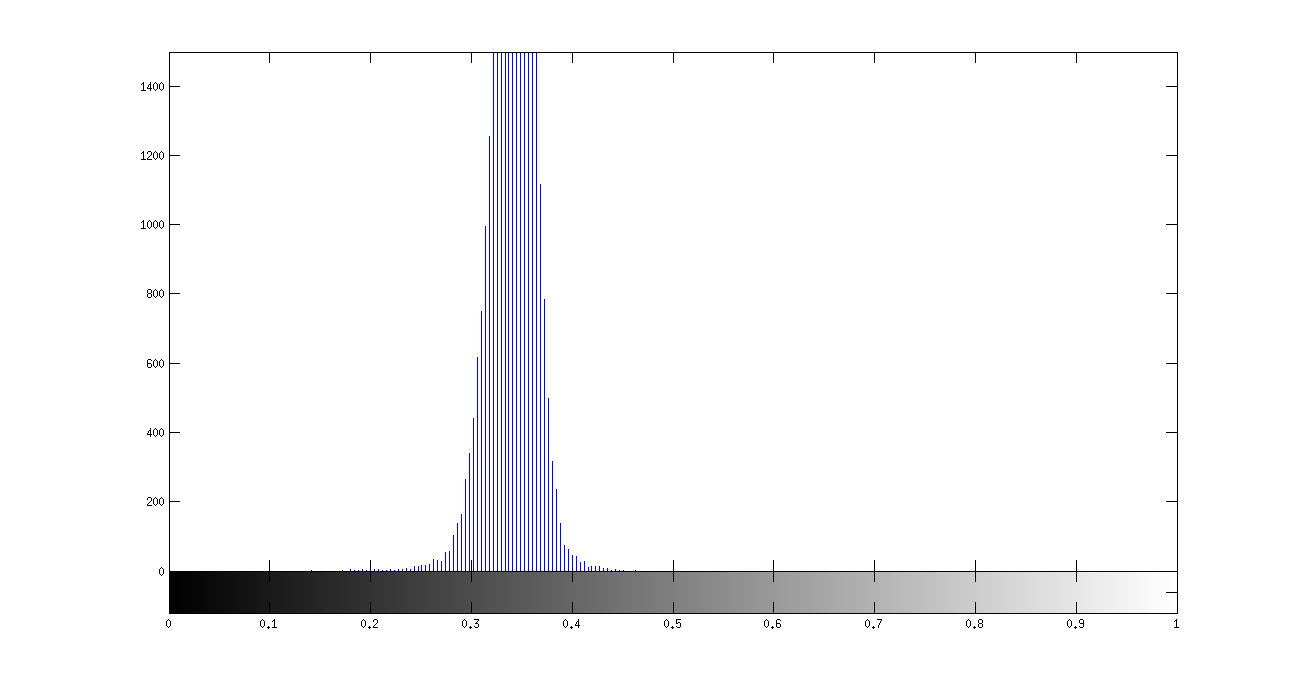
\includegraphics[width=6cm]{../th_hist}\\
Unfortinatly our solution is not perfect it will fail when \\%TODO 
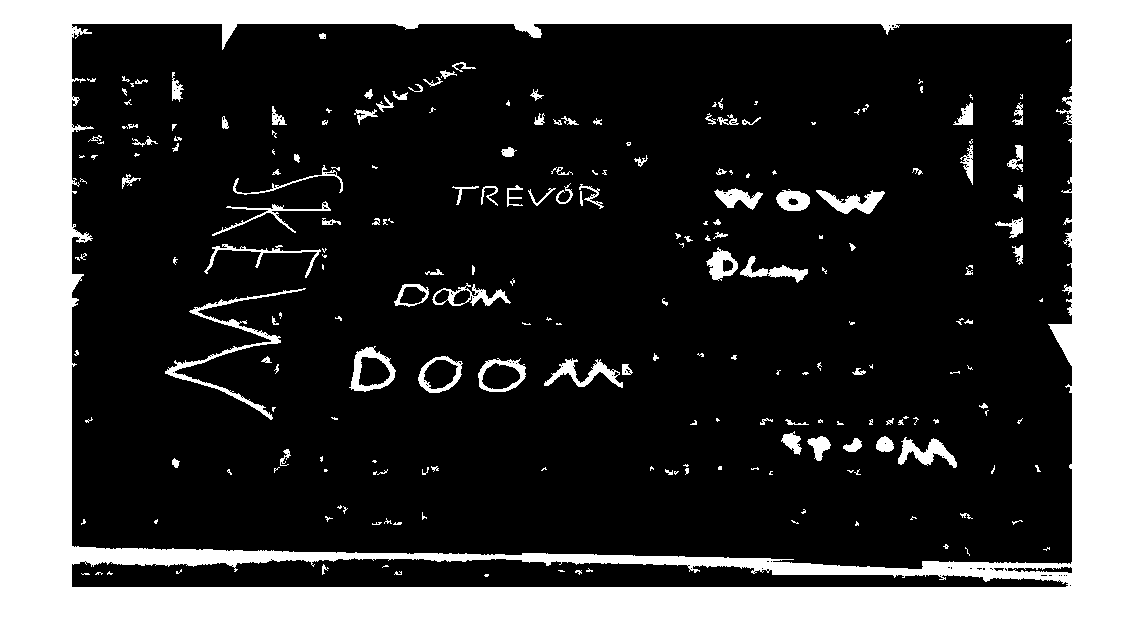
\includegraphics[width=6cm]{../thresh} %TODO picture of failure 
\\
};

\node (ref) [startstop, below of=step8,yshift=1cm, xshift=17cm] {{\huge Refrences}\\,\begin{verbatim}  %TODO format as bib 
http://yann.lecun.com/exdb/mnist/ 
http://www.gavo.t.u-tokyo.ac.jp/~qiao/database.html 
http://ieeexplore.ieee.org/stamp/stamp.jsp?arnumber=1315187
\end{verbatim}
%Chen, Huizhong, Sam S. Tsai, Georg Schroth, David M. Chen, Radek Grzeszczuk, and Bernd Girod. "ROBUST TEXT DETECTION IN NATURAL IMAGES WITH EDGE-ENHANCED MAXIMALLY STABLE EXTREMAL REGIONS." ROBUST TEXT DETECTION IN NATURAL IMAGES WITH EDGE-ENHANCED MAXIMALLY STABLE EXTREMAL REGIONS (n.d.): n. pag. Web. <http://web.stanford.edu/~hchen2/papers/ICIP2011_RobustTextDetection.pdf>.
%Coates,, Adam, Blake Carpenter, and Carl Case,. "Text Detection and Character Recognition in Scene Images with Unsupervised Feature Learning." Text Detection and Character Recognition in Scene Images with Unsupervised Feature Learning (n.d.): n. pag. Web. <http://ai.stanford.edu/~ang/papers/icdar01-TextRecognitionUnsupervisedFeatureLearning.pdf>.
%Epshtein, Boris, Eyal Ofek, and Yonatan Wexler. Detecting Text in Natural Scenes with Stroke Width Transform (n.d.): n. pag. Microsoft Corporation. Web.
%Koo,, Hyung Il, and Duck Hoon Kim,. "Scene Text Detection via Connected Component Clustering and Nontext Filtering." IEEE TRANSACTIONS ON IMAGE PROCESSING 22.6 (2013): 2296-305. Web. 1 Oct. 2014. <http://ieeexplore.ieee.org/stamp/stamp.jsp?arnumber=6471224&tag=1>.
%Yin, Xu-Cheng, Xuwang Yin, Kaizhu Huang, and Hong-Wei Hao. "Robust Text Detection in Natural Scene Images." (n.d.): n. pag. Web. <http://arxiv.org/pdf/1301.2628.pdf>.


};
\draw [arrow] (start) -- (step1);
\draw [arrow] (step1) -- (step2);
\draw [arrow] (step2) -- (step3);
\draw [arrow] (step3) -- (step4);
%\draw [arrow] (step4) -- (step5);
\draw [arrow] (step5) -- (step6);
\draw [arrow] (step6) -- (step7);
\draw [arrow] (step7) -- (step8);
\draw [arrow] (step8) -- (step9);



\end{tikzpicture}


%\centering
%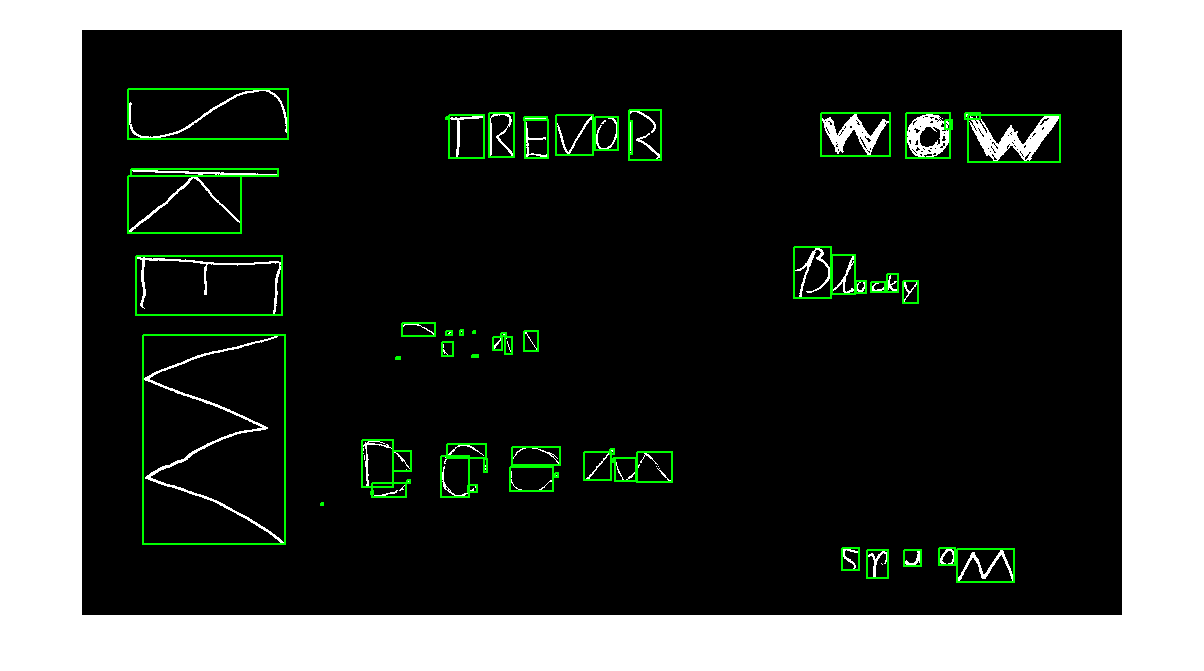
\includegraphics[width=2in]{../BoundingBoxImage_clean}
%\label{fig:BoundingBoxImage_clean}



%\centering 
%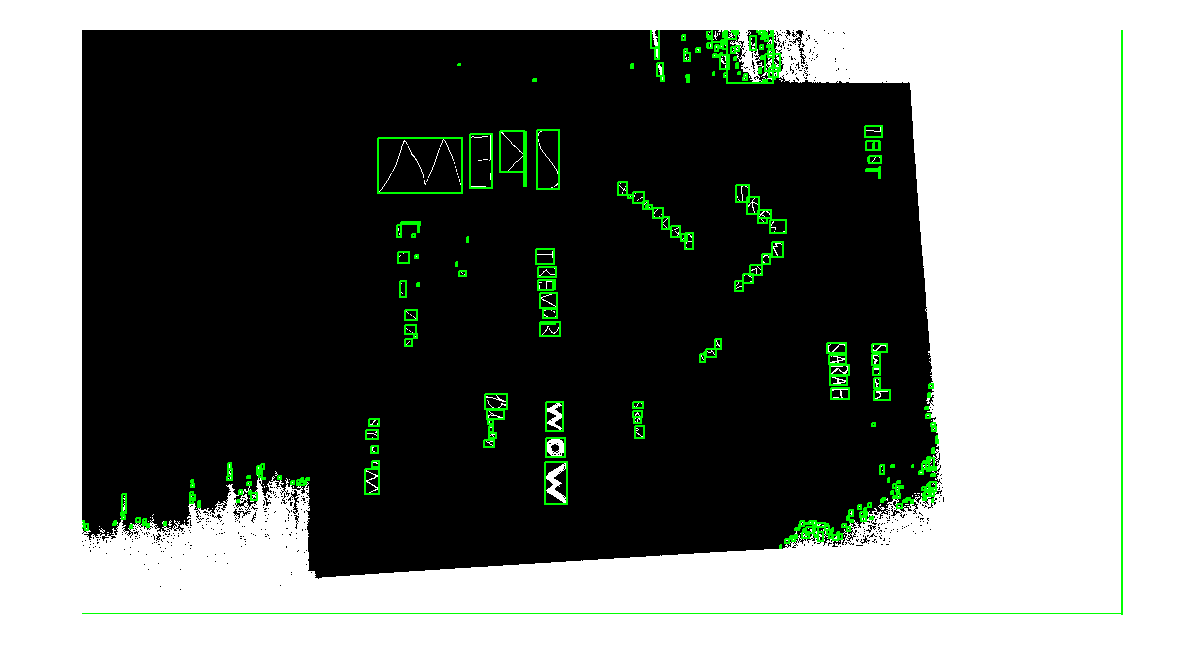
\includegraphics[width=2in]{../BoundingBoxImage_variedlighting}
%\label{fig:BoundingBoxImage_variedlighting}


%\centering
%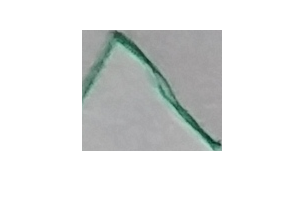
\includegraphics[width=2in]{../M_1}
%\label{fig:M_1}



%\centering
%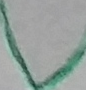
\includegraphics[width=2in]{../M_2}
%\label{fig:M_2}



%\centering
%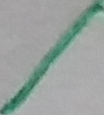
\includegraphics[width=2in]{../M_3}
%\label{fig:M_3}



%\centering
%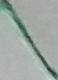
\includegraphics[width=2in]{../M_4}
%\label{fig:M_4}



%\centering
%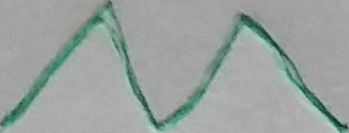
\includegraphics[width=2in]{../M_full}
%\label{fig:M_full}


%\centering
%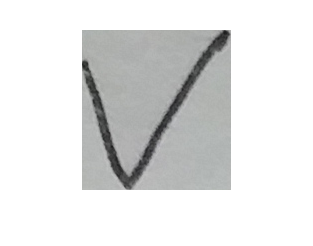
\includegraphics[width=2in]{../W_1}
%\label{fig:W_1}

% %refrences
%\begin{framed}
%{\large
%References}

%\end{framed}


\end{document}